%!TEX root = ../../../memoria.tex
\section{Carro Compra}
	El carro de compra agrupa todos los productos seleccionados para efectuar la compra. Actualmente del carro de compra se pueden desprender dos acciones: \nameref{chapter:section:carro_compra:subsection:add} y \nameref{chapter:section:carro_compra:subsection:request}.

	\subsection{Agregar elementos al carro}\label{chapter:section:carro_compra:subsection:add}

		El proceso de agregar elementos es muy sencillo, simplemente hay que ir a la vista de un producto, ir donde esta el botón \addtocartLABEL, seleccionar la cantidad de productos que se desean agregar y finalmente apretar el botón. En la \refFigura{figure:solution:cart:button} se han seleccionado 4 productos para agregar al carro. Este diseño ha sido inspirado también por el \websiteINT de \shopifyNAME (\refFigura{figure:productos:example:leifshop_product_section_add_to_cart}).

		\begin{figure}[H]
			\centering
			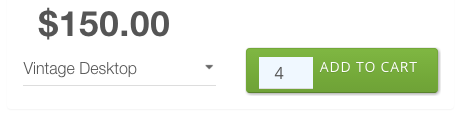
\includegraphics[width=0.8\textwidth]{figuras/productos/details/write/add_to_cart_button.png}
			\caption{Botón para agregar productos al carro. En la figura se han seleccionado 4 productos Vintage Desktop para agregar al carro de compra.}
			\label{figure:solution:cart:button}
		\end{figure}

		Es importante agregar que la opción \textit{Vintage Desktop} es la única opción disponible del sistema. Actualmente la plataforma no permite el ingreso de \VariantsForm para el mismo producto. Solo se construyo de esta manera para dar soporte cuando dicha funcionalidad sea implementada.

		Mostrar la confirmación de objeto agregado y permanecer en la misma página es algo fundamental. Las personas no han pedido moverse a otra página, de esta manera no hay sorpresas y se mantiene la buena experiencia. Además es posible que consideren agregar más productos al carro antes de \checkoutCOM \cite{online_official_conversionxl_checkout_flow}. Consideranto esto, se muestra una notificación en la parte superior de la pantalla sobre el ingreso del nuevo producto al carro sin abandonar la página actual (\refFigura{figure:solution:cart:add_motification}).

		\begin{figure}[H]
			\centering
			
\includegraphics[width=0.4\textwidth]{figuras/cart/ui/add_notification.png}
			\caption{\FeedbackCPT del nuevo producto agregado al carro.}
			\label{figure:solution:cart:add_motification}
		\end{figure}

		%TODO : ver si dejar esto o quitarlo. Agregar notificacion de feedback
		Usualmente el \textit{agregar al carro}, el botón con la acción final \websiteINT \ecommerceCOM cae en una de estas dos opciones: no está bien diseñado o no está ubicado estratégicamente para el uso del cliente \cite{online_official_usabilitygeek_guidelines_usability}. Por esta razón se creó un botón evidente, claro y prominente, en comparación a otras funcionalidades dentro de la misma página. Un ejemplo de lo que no se debe hacer se observa en la \refFigura{figure:apendice:productos:example:usabilitygeek_guidelines_wrong_ui_add_to_cart}.
		%Very often, the ‘Add to Cart’, the final action button in an e-Commerce website is either not well designed or strategically placed to grab prospective buyer’s action. The selection of shape, color, font typography, and button content all trigger the final action. Make sure the ‘Add to Cart’ button is obvious, bright, and prominent in comparison to other features on product page such as wishlists, view product, email to friend, or check out buttons. Less important functions should be lighter colored buttons or simple text links.

		\begin{figure}[H]
			\centering
			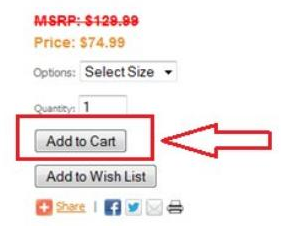
\includegraphics[width=0.3\textwidth]{figuras/productos/examples/usabilitygeek_guidelines_wrong_ui_add_to_cart.png}
			\caption{Mala práctica en el diseño del botón para agregar elementos al carro. Entre otros detalles el botón no tiene un diseño que lo distinga del botón agregar a la lista de deseos.}
			\label{figure:apendice:productos:example:usabilitygeek_guidelines_wrong_ui_add_to_cart}
		\end{figure}

		Una vez agregado al carro, el número de elementos presentes se actualiza. Este número es visible en la parte superior izquierda de la interfaz (\refFigura{figure:solution:cart:header}).

		\begin{figure}[H]
			\centering
			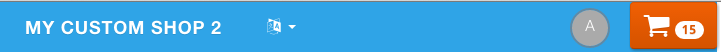
\includegraphics[width=0.8\textwidth]{figuras/header/toolbar/ui.png}
			\caption{Icono que muestra la cantidad de elementos que tiene el carro. El icono del carro es un botón para la vista del carro.}
			\label{figure:solution:cart:header}
		\end{figure}

		El estado del carro de compra se guarda en la base de datos, esto quiere decir que aunque haga \logoutCPT, el estado seguirá vigente para la próxima vez que haga \loginUpperCPT.


	\subsection{Consultar los elementos del carro}\label{chapter:section:carro_compra:subsection:request}

		%Por muy voluble que pueda parecer, las personas rápidamente abandonarán los carros de compra si no pueden localizar botones de \checkoutCOM inmediatamente \cite{online_official_imediaconnection_best_practices_shopping_cart}.
		% Include checkout buttons at the top and bottom of the screen
		% As fickle as it may seem, people will quickly abandon their shopping carts if they're unable to locate checkout buttons right away. Your shopping cart should make it as easy as possible for people to buy your products, so include checkout buttons at the top and bottom of the screen. Use A/B testing to figure out the most effective designs and colors too.
		% Read more at http://www.imediaconnection.com/content/36794.asp#6qlTEqOcCeTePmFQ.99


		Existen dos claves para un buen despliegue de contenido en un carro de compras \cite{online_official_conversionxl_checkout_flow}:
		\begin{itemize}
			\item
				\textbf{Claridad}. Que sea sencillo y obvio entender qué es lo que se tiene en el carro y su costo final, incluyendo \shipping e impuestos. Costos sorpresivos producen que los clientes abandonen los carros de compra \cite{online_official_conversionxl_checkout_flow}.
			\item
				\textbf{Control}. Es sencillo realizar cambios \cite{online_official_conversionxl_checkout_flow}. Esto incluye actualización de cantidad y eliminar productos \cite{online_official_conversionxl_shopping_cart_abandonment}.
		\end{itemize}

		El icono del carro de compras que se aprecia en la \refFigura{figure:solution:cart:header} es a su vez un botón, el cual muestra todos los elementos agregados al carro en una lista horizontal. Además muestra un resumen de la compra, inspirado en el que utiliza el sitio de \shopifyNAME (\refFigura{figure:apendice:cart:example:cart_summarize_shopify}), mostrando la siguiente información: 
		\begin{itemize}
			% \item
			% 	Cantidad de elementos.
			\item
				Subtotal.
			\item
				Costos de envío.
			\item
				Impuestos
			\item
				Total
		\end{itemize}

		Todos estos detalles, que se plasman en la \refFigura{figure:solution:cart:main} fueron diseñados con el fín de mantener \textbf{Claridad}.

		\begin{figure}[H]
			\centering
			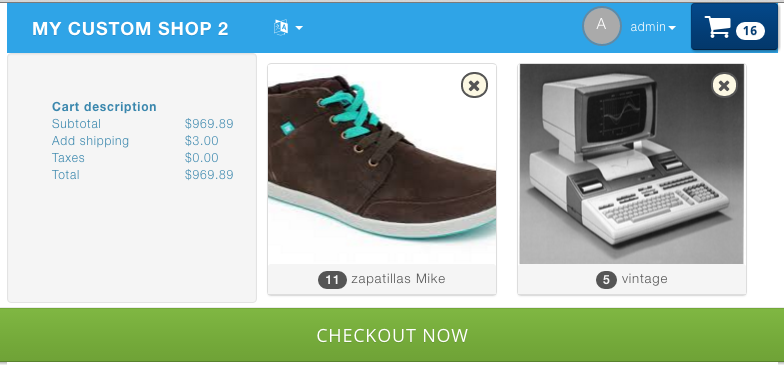
\includegraphics[width=0.8\textwidth]{figuras/cart/ui/main.png}
			\caption{Información global del carro. Tiene un resumen del costo total de los elementos seleccionados.}
			\label{figure:solution:cart:main}
		\end{figure}

		Cada uno de los diferentes elementos agregados al carro pueden ser eliminados simplemente presionando sobre la [x] que tiene asociada cada producto (\refFigura{figure:solution:cart:product}). Esto permite tener \textbf{control} sobre el contenido del carro. Es importante recordar como concepto general de diseño de interfaces, que es inevitable que las personas cometan errores, o incluso cambien de parecer durante algún procedimiento. Es necesario entonces permitir correcciones \cite{online_goodgui_org}. 

		\begin{figure}[H]
			\centering
			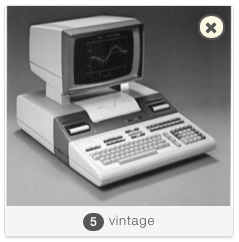
\includegraphics[width=0.5\textwidth]{figuras/cart/ui/cart_item.png}
			\caption{Vista básica de un producto seleccionado. La [x] permite eliminar ese producto del carro de compra.}
			\label{figure:solution:cart:product}
		\end{figure}

		El botón \checkoutNowLABEL que se ubica en la parte inferior de la vista \nameref{chapter:section:carro_compra:subsection:request} nos envía a la interfaz de \nameref{chapter:solucionimplementada:section:checkout}.

		De momento no es posible actualizar la cantidad de un determinado producto dentro del carro. En el caso particular del producto de la \refFigura{figure:solution:cart:product}, solo se pueden eliminar los 4 productos simultáneamente.

		Otra característica interesante que ha sido integrada, es de notificar al cliente cuando uno de sus productos esta bajo en \stockEF (\limitedStockEF) y sin \stockEF (\limitedStockEF).

		En la \refFigura{figure:cart:ui:cart_icon_warning} se aprecia como el botón del carro de compras a cambiado su color en relación al que aparece en la \refFigura{figure:solution:cart:main}. 

		\begin{figure}[H]
			\centering
			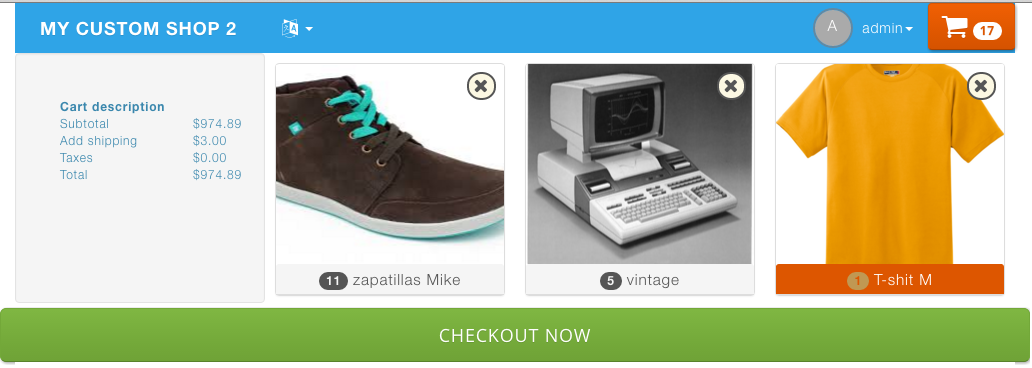
\includegraphics[width=0.8\textwidth]{figuras/cart/ui/cart_icon_warning.png}
			\caption{El botón del carro a cambiado de color. Esta informando que un producto esta con \limitedStockEF.}
			\label{figure:cart:ui:cart_icon_warning}
		\end{figure}

		También se aprecia que el producto \textit{T-shirt} esta dentro de un contenedor de color distinto en relación a los otros dos productos. Esto ocurre para identificar que ese producto es aquel que se encuentra con  \limitedStockEF. En la \refFigura{figure:cart:ui:item_warning} Se aprecia mejor el producto \textit{T-shirt}.

		\begin{figure}[H]
			\centering
			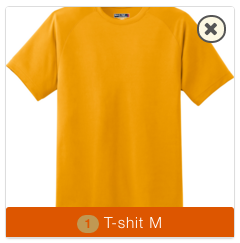
\includegraphics[width=0.5\textwidth]{figuras/cart/ui/item_warning.png}
			\caption{El contenedor del producto \textit{T-shirt} esta en amarillo. Esto indica que el producto esta con \limitedStockEF.}
			\label{figure:cart:ui:item_warning}
		\end{figure}
